% Created 2018-04-18 Wed 14:40
% Intended LaTeX compiler: pdflatex
\documentclass[10pt, compress, aspectratio=169, xcolor={table,usenames,dvipsnames}]{beamer}

\mode<beamer>{\usetheme[numbering=fraction, progressbar=none, titleformat=smallcaps, sectionpage=none]{metropolis}}
\usepackage{sourcecodepro}
\usepackage{booktabs}
\usepackage{array}
\usepackage{listings}
\usepackage{graphicx}
\usepackage[english]{babel}
\usepackage[scale=2]{ccicons}
\usepackage{url}
\usepackage{relsize}
\usepackage{amsmath}
\usepackage{bm}
\usepackage{wasysym}
\usepackage{ragged2e}
\usepackage{textcomp}
\usepackage{pgfplots}
\usepgfplotslibrary{dateplot}
\definecolor{Base}{HTML}{191F26}
\definecolor{Accent}{HTML}{157FFF}
\setbeamercolor{alerted text}{fg=Accent}
\setbeamercolor{frametitle}{bg=Base}
\setbeamercolor{normal text}{bg=black!2,fg=Base}
\setsansfont[BoldFont={Source Sans Pro Semibold},Numbers={OldStyle}]{Source Sans Pro}
\lstdefinelanguage{Julia}%
{morekeywords={abstract,struct,break,case,catch,const,continue,do,else,elseif,%
end,export,false,for,function,immutable,mutable,using,import,importall,if,in,%
macro,module,quote,return,switch,true,try,catch,type,typealias,%
while,<:,+,-,::,*,/},%
sensitive=true,%
alsoother={$},%
morecomment=[l]\#,%
morecomment=[n]{\#=}{=\#},%
morestring=[s]{"}{"},%
morestring=[m]{'}{'},%
}[keywords,comments,strings]%
\lstset{ %
backgroundcolor={},
basicstyle=\ttfamily\scriptsize,
breakatwhitespace=true,
breaklines=true,
captionpos=n,
commentstyle=\color{Accent},
escapeinside={\%*}{*)},
extendedchars=true,
frame=n,
keywordstyle=\color{Accent},
language=R,
rulecolor=\color{black},
showspaces=false,
showstringspaces=false,
showtabs=false,
stepnumber=2,
stringstyle=\color{gray},
tabsize=2,
}
\renewcommand*{\UrlFont}{\ttfamily\smaller\relax}
\graphicspath{{../img/}}
\addtobeamertemplate{block begin}{}{\justifying}
\usetheme{default}
\author{\footnotesize Pedro Bruel \newline \scriptsize \emph{phrb@ime.usp.br}}
\date{\scriptsize \today}
\title{Autotuning: A Design of Experiments Approach}
\hypersetup{
 pdfauthor={\footnotesize Pedro Bruel \newline \scriptsize \emph{phrb@ime.usp.br}},
 pdftitle={Autotuning: A Design of Experiments Approach},
 pdfkeywords={},
 pdfsubject={},
 pdfcreator={Emacs 25.3.1 (Org mode 9.1.9)}, 
 pdflang={English}}
\begin{document}

\maketitle
\begin{frame}{Outline}
\tableofcontents
\end{frame}


\section{Autotuning}
\label{sec:orgb0368a3}
\begin{frame}[fragile,label={sec:org30cfdab}]{Autotuning: Optimizing Program Configurations}
 \begin{columns}
\begin{column}{0.5\columnwidth}
\begin{block}{Architectures for High Performance Computing}
\begin{center}
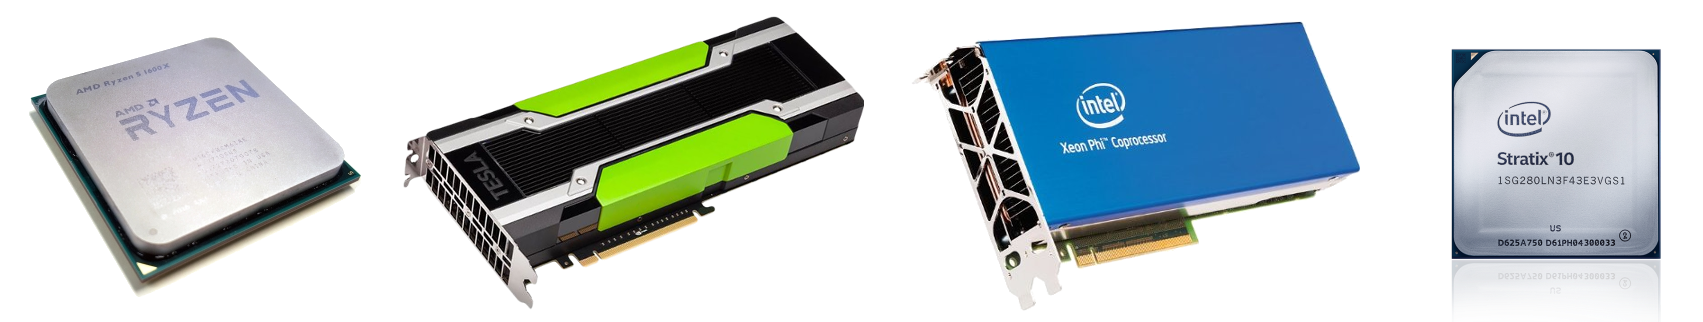
\includegraphics[width=.9\linewidth]{../img/architectures.png}
\end{center}

How to write \alert{efficient code} for each of these?

\begin{block}{Autotuning}
\vspace{.2cm}

The process of \alert{automatically finding} a \alert{configuration} of a program that
optimizes an \alert{objective}
\end{block}
\end{block}
\end{column}

\begin{column}{0.5\columnwidth}
\begin{block}{Configurations}
\begin{itemize}
\item Program Configuration
\begin{itemize}
\item Algorithm, block size, \(\dots\)
\end{itemize}
\item Source code transformation
\begin{itemize}
\item Loop unrolling, tiling, rotation \(\dots\)
\end{itemize}
\item Compiler configuration
\begin{itemize}
\item \texttt{-O2}, vectorization, \(\dots\)
\end{itemize}
\item \(\dots\)
\end{itemize}

\begin{block}{Objectives}
\begin{itemize}
\item Execution time
\item Memory \& power consumption
\item \(\dots\)
\end{itemize}
\end{block}
\end{block}
\end{column}
\end{columns}
\end{frame}

\begin{frame}[label={sec:org60a4207}]{Autotuning: Search Spaces}
\begin{columns}
\begin{column}{0.5\columnwidth}
\begin{block}{Search Spaces}
\vspace{.2cm}

Represent the \alert{effect} of all possible
\alert{configurations} on the \alert{objectives}

Can be difficult to explore, with multiple \alert{local optima}
and \alert{undefined regions}
\end{block}
\end{column}

\begin{column}{0.5\columnwidth}
\begin{center}
\begin{center}
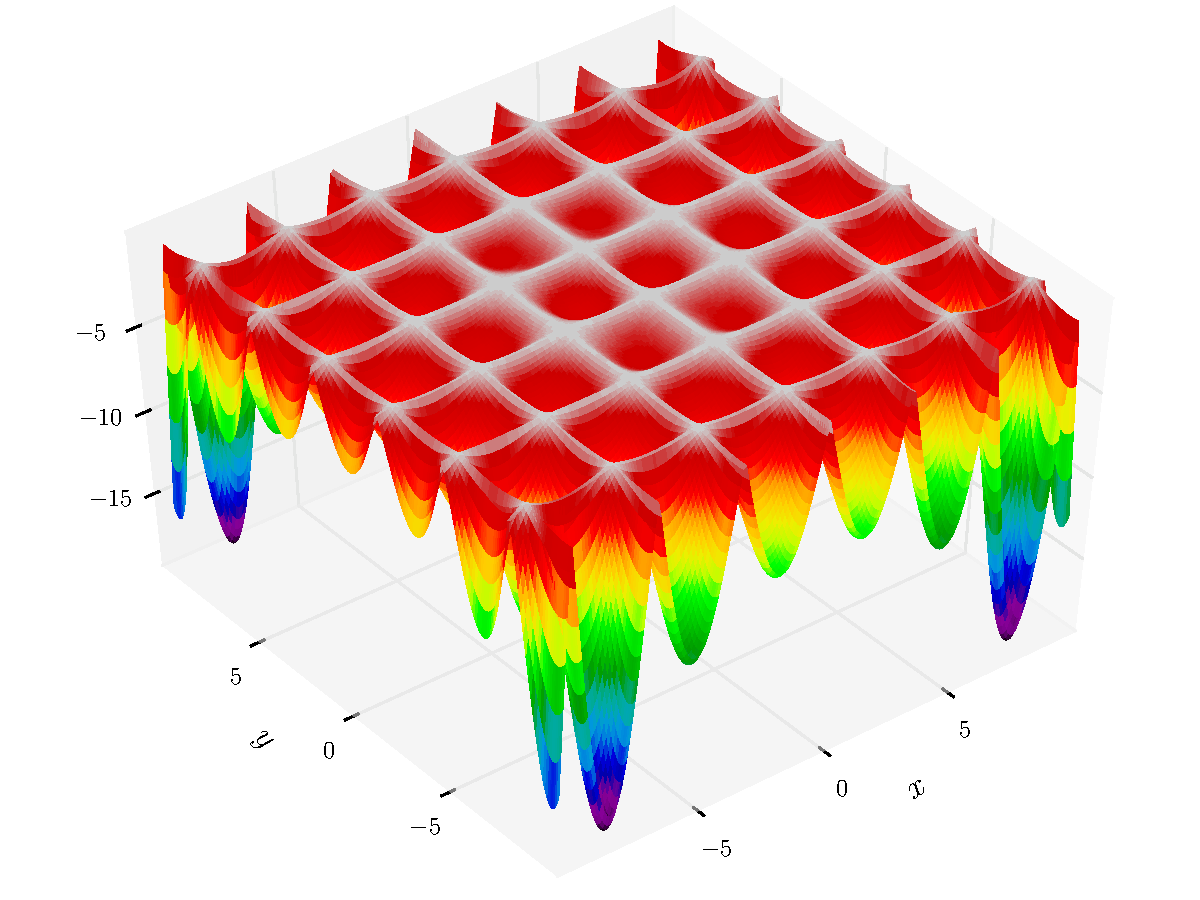
\includegraphics[width=.9\linewidth]{../img/holder_table.pdf}
\end{center}    

\alert{Hölder Table Function}
\end{center}
\end{column}
\end{columns}
\end{frame}

\begin{frame}[label={sec:org1f2b070}]{Autotuning: Exploring Search Spaces}
\begin{columns}
\begin{column}{0.5\columnwidth}
\begin{block}{Issue 1: \alert{Exponential Growth}}
\vspace{.2cm}

\alert{Simple factors} can generate \alert{large spaces}:

\begin{itemize}
\item 30 \alert{boolean} factors
\item \(2^{30}\) combinations
\end{itemize}

\begin{block}{Issue 2: \alert{Geometry}}
\begin{itemize}
\item \alert{Discrete} or \alert{continous} factors
\item \alert{``Smoothness''}
\item \alert{Interactions} between factors
\end{itemize}
\end{block}
\end{block}
\end{column}

\begin{column}{0.5\columnwidth}
\begin{block}{Issue 3: \alert{Measurement Time}}
\vspace{.2cm}

Time to \alert{compile}:

\begin{itemize}
\item \alert{Benchmark} GPU applications: \alert{1\textasciitilde{}10s}
\item \alert{Benchmark} FPGA applications: \alert{1\textasciitilde{}10min}
\item \alert{Industrial} FPGA applications: \alert{1\textasciitilde{}10h}
\end{itemize}
\end{block}
\end{column}
\end{columns}
\end{frame}
\begin{frame}[label={sec:orgec6e0e8}]{Autotuning: Multiple Approaches}
\begin{columns}
\begin{column}{0.5\columnwidth}
\begin{block}{Popular Approaches}
\footnotesize
\begin{itemize}
\item \colorbox{red!25}{Exhaustive}
\item \colorbox{green!25}{Meta-Heuristics}
\item \colorbox{cyan!25}{Machine Learning}
\end{itemize}
\normalsize

\vspace{-.4cm}

\begin{table}
    \centering
    \scriptsize
    \begin{tabular}{@{}lll@{}}
        \toprule
        System & Domain & Approach \\ \midrule
        \rowcolor{red!25} ATLAS & Dense Linear Algebra & Exhaustive\\ \addlinespace
        \rowcolor{green!25} INSIEME & Compiler & Genetic Algorithm \\
        \rowcolor{green!25} Active Harmony & Runtime & Nelder-Mead \\
        \rowcolor{green!25} ParamILS & Domain-Agnostic & Stochastic Local Search \\
        \rowcolor{green!25} OPAL & Domain-Agnostic & Direct Search \\
        \rowcolor{green!25} OpenTuner & Domain-Agnostic & Ensemble \\ \addlinespace
        \rowcolor{cyan!25} MILEPOST GCC & Compiler & Machine Learning \\
        \rowcolor{cyan!25} Apollo & GPU kernels & Decision Trees \\ \addlinespace
        \bottomrule
    \end{tabular}
\end{table}

\end{block}
\end{column}

\begin{column}{0.5\columnwidth}
\begin{block}{Main Issues}
\begin{itemize}
\item These approaches \alert{assume}:
\begin{itemize}
\item A \alert{large number of function evaluations}
\item Seach space \alert{``smoothness''}
\item Good solutions are \alert{reachable}
\end{itemize}
\item After optimizing:
\begin{itemize}
\item \alert{Learn nothing} about the search space
\item \alert{Can't explain} why optimizations work
\end{itemize}
\end{itemize}
\end{block}
\end{column}
\end{columns}
\end{frame}
\section{Applying Design of Experiments to Autotuning}
\label{sec:orgfe58fa6}
\begin{frame}[label={sec:org5ac00d2}]{Applying Design of Experiments to Autotuning}
\begin{columns}
\begin{column}{0.5\columnwidth}
\begin{block}{Our Approach}
\vspace{.2cm}

Using \alert{efficient experimental design} to overcome issues
related to \alert{exponential growth}, \alert{geometry}, and
\alert{measurement time}

\begin{block}{Design Requirements}
\begin{itemize}
\item Support a large number of factors (\alert{Exponential Growth})
\item Support numerical and categorical factors (\alert{Geometry})
\item Minimize function evaluations (\alert{Measurement Time})
\end{itemize}
\end{block}
\end{block}
\end{column}

\begin{column}{0.5\columnwidth}
\begin{block}{Main Design Candidates}
\vspace{.2cm}

\alert{Screening} designs:

\begin{itemize}
\item Estimate \alert{main effects}
\item Aim to \alert{minimize runs}
\item Assume \alert{interactions are negligible}
\end{itemize}

\alert{Mixed-Level} designs:

\begin{itemize}
\item Factors have \alert{different numbers of levels}
\item Many \alert{optimality criteria}
\end{itemize}
\end{block}
\end{column}
\end{columns}
\end{frame}

\begin{frame}[label={sec:org1508f12}]{Screening Designs}
\begin{columns}
\begin{column}{0.5\columnwidth}
\vspace{.4cm}

A Plackett-Burman \alert{screening design} for \(7\)
\alert{2-level factors}:

\vspace{.2cm}

\begin{table}[]
    \centering
    \begin{tabular}{@{\kern\tabcolsep}cccccccc@{\kern\tabcolsep}}
        \toprule
        Run & A & B & C & D & E & F & G \\ \midrule
        \cellcolor{gray!18}1 & \cellcolor{green!25}1 & \cellcolor{red!25}-1 & \cellcolor{green!25}1 & \cellcolor{red!25}-1 & \cellcolor{red!25}-1 & \cellcolor{green!25}1 & \cellcolor{green!25}1 \\
        \cellcolor{gray!18}2 & \cellcolor{green!25}1 & \cellcolor{green!25}1 & \cellcolor{green!25}1 & \cellcolor{red!25}-1 & \cellcolor{green!25}1 & \cellcolor{red!25}-1 & \cellcolor{red!25}-1 \\
        \cellcolor{gray!18}3 & \cellcolor{red!25}-1 & \cellcolor{green!25}1 & \cellcolor{red!25}-1 & \cellcolor{red!25}-1 & \cellcolor{green!25}1 & \cellcolor{green!25}1 & \cellcolor{green!25}1 \\
        \cellcolor{gray!18}4 & \cellcolor{red!25}-1 & \cellcolor{green!25}1 & \cellcolor{green!25}1 & \cellcolor{green!25}1 & \cellcolor{red!25}-1 & \cellcolor{green!25}1 & \cellcolor{red!25}-1 \\
        \cellcolor{gray!18}5 & \cellcolor{green!25}1 & \cellcolor{red!25}-1 & \cellcolor{red!25}-1 & \cellcolor{green!25}1 & \cellcolor{green!25}1 & \cellcolor{green!25}1 & \cellcolor{red!25}-1 \\
        \cellcolor{gray!18}6 & \cellcolor{green!25}1 & \cellcolor{green!25}1 & \cellcolor{red!25}-1 & \cellcolor{green!25}1 & \cellcolor{red!25}-1 & \cellcolor{red!25}-1 & \cellcolor{green!25}1 \\
        \cellcolor{gray!18}7 & \cellcolor{red!25}-1 & \cellcolor{red!25}-1 & \cellcolor{green!25}1 & \cellcolor{green!25}1 & \cellcolor{green!25}1 & \cellcolor{red!25}-1 & \cellcolor{green!25}1 \\
        \cellcolor{gray!18}8 & \cellcolor{red!25}-1 & \cellcolor{red!25}-1 & \cellcolor{red!25}-1 & \cellcolor{red!25}-1 & \cellcolor{red!25}-1 & \cellcolor{red!25}-1 & \cellcolor{red!25}-1  \\ \bottomrule
    \end{tabular}
\end{table}

\end{column}

\begin{column}{0.5\columnwidth}
\begin{block}{Screening Designs}
\vspace{.2cm}

\alert{Plackett-Burman} designs for \alert{2-level factors}:

\begin{itemize}
\item \alert{Orthogonal arrays} of \alert{strength \(2\)}
\item Estimate the \alert{main effects} of \alert{\(n\) factors with \(n + 1\) runs}
\end{itemize}

Construction:

\begin{itemize}
\item For \alert{\(n + 1\) multiple of \(4\)}
\item Identical to a fractional design if \alert{\(n + 1\) is a power of two}
\end{itemize}
\end{block}
\end{column}
\end{columns}
\end{frame}

\begin{frame}[label={sec:orgcece045}]{Looking at Data: CUDA Compiler Flags}
\begin{columns}
\begin{column}{0.3\columnwidth}
\begin{block}{CUDA Compiler Flags}
\begin{itemize}
\item \alert{Rodinia benchmark}
\item \alert{15} factors, \alert{few with multiple levels}
\item \alert{\(10^6\)} combinations
\item \alert{1\textasciitilde{}10s} to measure
\item \alert{Screening experiment}:
\begin{itemize}
\item \alert{15 ``2-level''} factors
\item \alert{4 ``dummy''} factors
\end{itemize}
\end{itemize}
\end{block}
\end{column}
\begin{column}{0.7\columnwidth}
\begin{center}
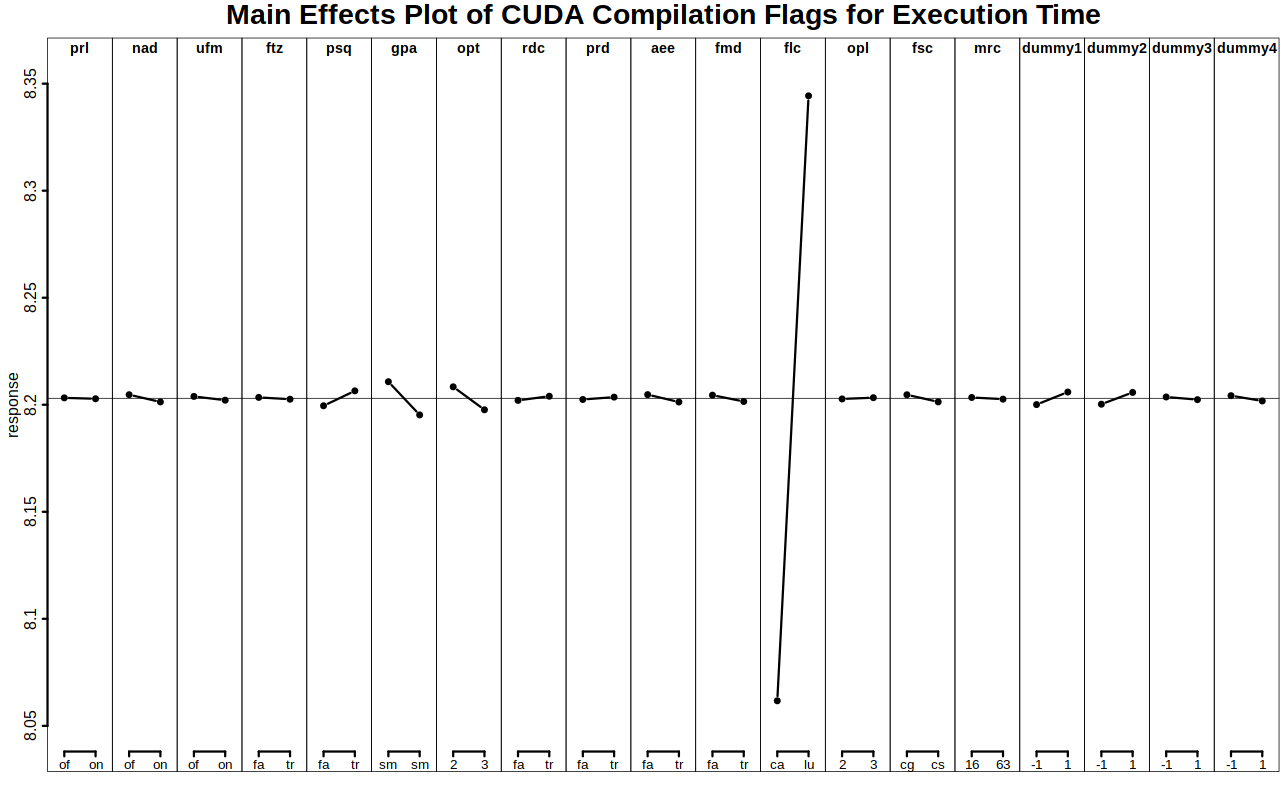
\includegraphics[width=.9\linewidth]{../img/main_effects_gpu.png}
\end{center}
\end{column}
\end{columns}
\end{frame}

\begin{frame}[label={sec:org08f4a01}]{Mixed-Level Designs}
\begin{columns}
\begin{column}{0.5\columnwidth}
\vspace{.1cm}

A \alert{multi-level} design for \(1\) \alert{2-level factor}
and \(3\) \alert{3-level factors}:

\vspace{-.3cm}

\begin{table}[]
    \scriptsize
    \centering
    \begin{tabular}{@{}ccccc@{}}
        \toprule
        Run & A & B & C & D \\ \midrule
        \cellcolor{gray!18}1 & \cellcolor{green!25}1 & \cellcolor{green!25}1 & \cellcolor{green!25}1 & \cellcolor{red!25}3 \\
        \cellcolor{gray!18}2 & \cellcolor{green!25}1 & \cellcolor{green!25}1 & \cellcolor{cyan!25}2 & \cellcolor{green!25}1 \\
        \cellcolor{gray!18}3 & \cellcolor{green!25}1 & \cellcolor{green!25}1 & \cellcolor{red!25}3 & \cellcolor{cyan!25}2 \\
        \cellcolor{gray!18}4 & \cellcolor{green!25}1 & \cellcolor{cyan!25}2 & \cellcolor{green!25}1 & \cellcolor{cyan!25}2 \\
        \cellcolor{gray!18}5 & \cellcolor{green!25}1 & \cellcolor{cyan!25}2 & \cellcolor{cyan!25}2 & \cellcolor{red!25}3 \\
        \cellcolor{gray!18}6 & \cellcolor{green!25}1 & \cellcolor{cyan!25}2 & \cellcolor{red!25}3 & \cellcolor{green!25}1 \\
        \cellcolor{gray!18}7 & \cellcolor{green!25}1 & \cellcolor{red!25}3 & \cellcolor{green!25}1 & \cellcolor{green!25}1 \\
        \cellcolor{gray!18}8 & \cellcolor{green!25}1 & \cellcolor{red!25}3 & \cellcolor{cyan!25}2 & \cellcolor{cyan!25}2 \\
        \cellcolor{gray!18}9 & \cellcolor{green!25}1 & \cellcolor{red!25}3 & \cellcolor{red!25}3 & \cellcolor{red!25}3 \\
        \cellcolor{gray!18}10 & \cellcolor{cyan!25}2 & \cellcolor{green!25}1 & \cellcolor{green!25}1 & \cellcolor{green!25}1 \\
        \cellcolor{gray!18}11 & \cellcolor{cyan!25}2 & \cellcolor{green!25}1 & \cellcolor{cyan!25}2 & \cellcolor{cyan!25}2 \\
        \cellcolor{gray!18}12 & \cellcolor{cyan!25}2 & \cellcolor{green!25}1 & \cellcolor{red!25}3 & \cellcolor{red!25}3 \\
        \cellcolor{gray!18}13 & \cellcolor{cyan!25}2 & \cellcolor{cyan!25}2 & \cellcolor{green!25}1 & \cellcolor{red!25}3 \\
        \cellcolor{gray!18}14 & \cellcolor{cyan!25}2 & \cellcolor{cyan!25}2 & \cellcolor{cyan!25}2 & \cellcolor{green!25}1 \\
        \cellcolor{gray!18}15 & \cellcolor{cyan!25}2 & \cellcolor{cyan!25}2 & \cellcolor{red!25}3 & \cellcolor{cyan!25}2 \\
        \cellcolor{gray!18}16 & \cellcolor{cyan!25}2 & \cellcolor{red!25}3 & \cellcolor{green!25}1 & \cellcolor{cyan!25}2 \\
        \cellcolor{gray!18}17 & \cellcolor{cyan!25}2 & \cellcolor{red!25}3 & \cellcolor{cyan!25}2 & \cellcolor{red!25}3 \\
        \cellcolor{gray!18}18 & \cellcolor{cyan!25}2 & \cellcolor{red!25}3 & \cellcolor{red!25}3 & \cellcolor{green!25}1 \\ \bottomrule
    \end{tabular}
\end{table}

\end{column}

\begin{column}{0.5\columnwidth}
\begin{block}{Mixed-Level Designs}
\begin{block}{Strategy 1: \alert{Contractive Replacement}}
\begin{itemize}
\item Find \alert{specific sets of \(k\)-level columns} of a design,
\alert{contract} the set into a new \alert{factor of with more levels}
\item \alert{Maintain orthogonality} of the design
\end{itemize}
\end{block}

\begin{block}{Strategy 2: \alert{Direct Construction}}
\vspace{.2cm}

Directly generate \alert{small mixed-level designs} by
solving \alert{Mixed Integer Programming problems}
\end{block}

\begin{block}{Strategy 3: \alert{D-Optimal Designs}}
\end{block}
\end{block}
\end{column}
\end{columns}
\end{frame}

\begin{frame}[label={sec:org7986337}]{Looking at Data: FPGA Compiler Parameters}
\begin{columns}
\begin{column}{0.4\columnwidth}
\begin{block}{FPGA Compiler Parameters}
\begin{itemize}
\item \alert{CHStone benchmark}
\item \alert{141} factors, \alert{most with multiple levels}
\item \alert{\(10^{128}\)} combinations
\item \alert{1\textasciitilde{}10min} to measure
\item \alert{Multiple objectives}
\item \alert{Search with meta-heuristics}:
\begin{itemize}
\item \alert{Unstructured data difficults analysis}
\item We are working on \alert{obtaining more data}
\end{itemize}
\end{itemize}
\end{block}
\end{column}
\begin{column}{0.6\columnwidth}
\begin{center}
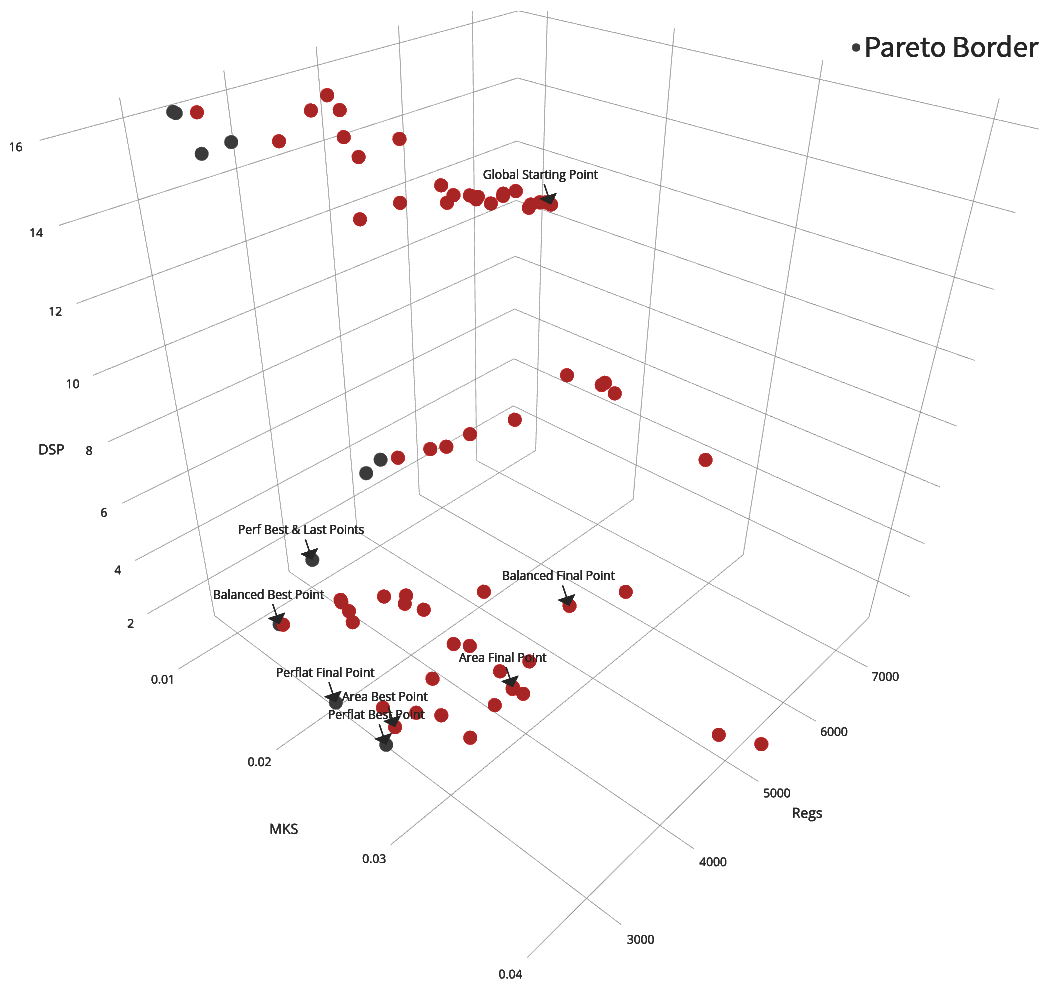
\includegraphics[width=.9\linewidth]{../img/fpga_space.png}
\end{center}
\end{column}
\end{columns}
\end{frame}
\section{Design Efficiency}
\label{sec:org004e58e}
\begin{frame}[label={sec:orga3c692a}]{Design Efficiency: Introduction}
\begin{columns}
\begin{column}{0.5\columnwidth}
\begin{block}{Linear Regression Model}
\vspace{.2cm}

A simple \alert{regression model}:

\begin{center}
\(y = \beta_{0} + \beta_{1}x_{1} + \dots + \beta_{k}x_{k} + \epsilon\)
\end{center}

We want to \alert{estimate} \(\beta_{0,\dots,k}\):

\begin{itemize}
\item Using \(n > k\) \alert{observations} \(y_{1,\dots,n}\)
\item \alert{Distinct} \(x_{i1,\dots,ik}, \; i = 1,\dots,n\)
\end{itemize}

We will use \(n\) \alert{experiments} such as:

\begin{center}
\(y_{i} = \beta_{0} + \beta_{1}x_{i1} + \dots + \beta_{k}x_{ik} + \epsilon_{i}\)
\end{center}
\end{block}
\end{column}
\begin{column}{0.5\columnwidth}
\begin{block}{Least Squares Method}
\vspace{.2cm}

Writing in \alert{matrix form} we get:

\begin{center}
\(\mathbf{Y} = \mathbf{X}\bm{\beta} + \bm{\epsilon}\)
\end{center}

The \alert{least squares method} aims to minimize:
\vspace{-.7cm}
\begin{center}
\begin{align*}
L =& \; \sum\limits^{n}_{i = 1}{\epsilon_{i}^{2}}
= \bm{\epsilon}^{\prime}\bm{\epsilon}
= (\mathbf{Y} - \bm{X}\bm{\beta})^{\prime}(\mathbf{Y} - \bm{X}\bm{\beta}) = \\
=& \; \bm{Y}^{\prime}\bm{Y}
\; \colorbox{cyan!25}{$- \bm{\beta}^{\prime}\bm{X}^{\prime}\bm{Y} -
\bm{Y}^{\prime}\bm{X\beta}$} +
\bm{\beta}^{\prime}\bm{X}^{\prime}\bm{X\beta} = \\
=& \; \bm{Y}^{\prime}\bm{Y} \;
\colorbox{cyan!25}{$- 2\bm{\beta}^{\prime}\bm{X}^{\prime}\bm{Y}$} +
\bm{\beta}^{\prime}\bm{X}^{\prime}\bm{X\beta}
\end{align*}
\end{center}
\end{block}
\end{column}
\end{columns}
\end{frame}
\begin{frame}[label={sec:org25d0ad4}]{Design Efficiency: Estimating Model Coefficients}
\begin{columns}
\begin{column}{0.5\columnwidth}
\begin{block}{Minimizing Least Squares}
\vspace{.2cm}

The \alert{least squares method} aims to minimize:
\vspace{-.8cm}
\begin{center}
\begin{equation*}
L = \bm{Y}^{\prime}\bm{Y} - 2\bm{\beta}^{\prime}\bm{X}^{\prime}\bm{Y} +
\bm{\beta}^{\prime}\bm{X}^{\prime}\bm{X\beta}
\end{equation*}
\end{center}

\alert{Derivative} with respect to \(\bm{\beta}\), \alert{evaluated} at \(\bm{\hat{\beta}}\):
\vspace{-.7cm}
\begin{center}
\begin{equation*}
\left. \dfrac{\partial{}L}{\partial{}\bm{\beta}}\right|_{\bm{\hat{\beta}}} =
- 2\bm{X}^{\prime}\bm{Y} + 2\bm{X}^{\prime}\bm{X\hat{\beta}} = 0
\end{equation*}
\end{center}
Where \(\bm{\hat{\beta}}\) is an \alert{estimator} of \(\bm{\beta}\)
\end{block}
\end{column}
\begin{column}{0.5\columnwidth}
\begin{block}{Computing \(\bm{\hat{\beta}}\)}
\vspace{.2cm}

The previous equation simplifies to:
\vspace{-.8cm}
\begin{center}
\begin{equation*}
\bm{\hat{\beta}} = \left(\bm{X}^{\prime}\bm{X}\right)^{-1}\bm{X}^{\prime}\bm{Y}
\end{equation*}
\end{center}

The \alert{estimator} \(\bm{\hat{\beta}}\) is \alert{proportional} to
\(\left(\bm{X}^{\prime}\bm{X}\right)^{-1}\)
\begin{block}{Dispersion or Covariance Matrix}
\begin{itemize}
\item \alert{Information matrix}: \(\bm{X}^{\prime}\bm{X}\)
\item \alert{Dispersion} or \alert{Covariance matrix}: \(\left(\bm{X}^{\prime}\bm{X}\right)^{-1}\)
\end{itemize}
\end{block}
\end{block}
\end{column}
\end{columns}
\end{frame}
\begin{frame}[label={sec:orgf06ff44}]{Design Efficiency: The Dispersion Matrix}
\begin{columns}
\begin{column}{0.5\columnwidth}
\begin{block}{Interpreting Eigenvalues of \(\left(\bm{X}^{\prime}\bm{X}\right)^{-1}\)}
\vspace{.2cm}

A design \(D_{n,2}\) will have a \(3\times3\) \alert{dispersion matrix}, if we assume
\alert{linear relationships} and no \alert{factor interactions}

\begin{center}
\includegraphics[width=.9\linewidth]{./pdf/3dshape.pdf}
\end{center}
\end{block}
\end{column}

\begin{column}{0.5\columnwidth}
\begin{block}{Efficiency Metrics based on \(\left(\bm{X}^{\prime}\bm{X}\right)^{-1}\)}
\begin{block}{A-Efficiency}
\vspace{-.8cm}
\begin{center}
\begin{equation*}
A_{eff} = \left(n \times \text{tr}\left(\left(\bm{X}^{\prime}\bm{X}\right)^{-1}\right)/k\right)^{(-1)}
\end{equation*}
\end{center}

\vspace{-.6cm}
\begin{itemize}
\item \alert{Arithmetic mean} of \alert{eigenvalues} of \(\left(\bm{X}^{\prime}\bm{X}\right)^{-1}\)
\end{itemize}
\vspace{-.3cm}
\end{block}
\begin{block}{D-Efficiency}
\vspace{-.8cm}
\begin{center}
\begin{equation*}
D_{eff} = \left(n \times \left|\left(\bm{X}^{\prime}\bm{X}\right)^{-1}\right|^{1/k}\right)^{(-1)}
\end{equation*}
\end{center}

\vspace{-.6cm}
\begin{itemize}
\item \alert{Geometric mean} of \alert{eigenvalues} of \(\left(\bm{X}^{\prime}\bm{X}\right)^{-1}\)
\end{itemize}
\vspace{-.3cm}
\end{block}
\begin{block}{G-Efficiency}
\end{block}
\end{block}
\end{column}
\end{columns}
\end{frame}

\begin{frame}[fragile,label={sec:orgb6be2a3}]{D-Optimal Designs: Example}
 \begin{columns}
\begin{column}{0.5\columnwidth}
\begin{block}{Example}
\begin{itemize}
\item Factors \& Levels: \(\mathbf{X} = \{x_1 = \{1, 2, 3\}, x_2 = \{1, 2, 3\}\}\)
\item Model: \(\mathbf{Y} = \mathbf{X}\beta + \eta\)
\item Minimize: \alert{D-optimality}
\item Candidate set: \alert{Full factorial}
\item Selection method: \alert{Federov's algorithm}
\end{itemize}

\begin{block}{Source code}
\lstset{language=r,label= ,caption= ,captionpos=b,numbers=none}
\begin{lstlisting}
library(AlgDesign)
full_factorial <- gen.factorial(c(3, 3),
                      factors = c(1, 2))
output <- optFederov(~., full_factorial,
                     nTrials = 5)
\end{lstlisting}
\end{block}
\end{block}
\end{column}

\begin{column}{0.5\columnwidth}
\begin{block}{Output}
\scriptsize

\begin{verbatim}
$D
[1] 0.2

$A
[1] 11

$Ge
[1] 0.333

$Dea
[1] 0.135

$design
   1   4   5   6   9  
X1 "1" "1" "2" "3" "3"
X2 "1" "2" "2" "2" "3"

$rows
[1] 1 4 5 6 9
\end{verbatim}

\normalsize
\end{block}
\end{column}
\end{columns}
\end{frame}
\section{Perspectives}
\label{sec:orge6172d1}
\begin{frame}[label={sec:org2c5ca1d}]{Perspectives}
\begin{columns}
\begin{column}{0.5\columnwidth}
\begin{block}{Perspectives}
\begin{block}{\alert{Short Term}}
\begin{itemize}
\item Study \alert{small}, \alert{balanced}, \alert{orthogonal} and
\alert{multi-level} designs for \alert{large numbers of factors}
\item Iteratively \alert{drop least significant factors} with
\alert{user input}
\end{itemize}
\end{block}

\begin{block}{\alert{Long Term}}
\begin{itemize}
\item Use such designs to \alert{autotune industrial-level FPGA applications}
\item Provide an \alert{autotuning shared library} to applications
\end{itemize}
\end{block}
\end{block}
\end{column}

\begin{column}{0.5\columnwidth}
\begin{block}{Takeaway}
\begin{block}{Target Scenario: \alert{FPGA Compiler Parameters}}
\begin{itemize}
\item \alert{Large search space}
\item \alert{Large measurement time}
\item Factors with \alert{multiple levels}
\end{itemize}

\vspace{-.3cm}
\end{block}

\begin{block}{Our Approach}
\vspace{.2cm}

Using \alert{efficient experimental designs} to overcome issues related
to \alert{exponential growth}, \alert{geometry}, and \alert{measurement time}
\end{block}

\begin{block}{Main Design Candidates}
\vspace{.2cm}

\alert{D-Optimal multi-level} designs
\end{block}
\end{block}
\end{column}
\end{columns}
\end{frame}

\maketitle
\end{document}
